%%
%% copyright quintard julien
%% 
%% kaneton
%% 
%% kaneton.tex
%% 
%% path          /home/mycure/kaneton/view/cursus/schedule
%% 
%% made by mycure
%%         quintard julien   [quinta_j@epita.fr]
%% 
%% started on    Mon Feb 21 16:02:54 2005   mycure
%% last update   Mon Oct 31 22:26:58 2005   mycure
%%

\documentclass[10pt,a4wide]{article}
\usepackage[english]{babel}
\usepackage{a4wide}
\usepackage[dvips]{graphicx}
\usepackage{graphics}
\usepackage{fancyheadings}
\pagestyle{fancy}

\bibliographystyle{plain}

\lhead{\scriptsize{kaneton project}}
\rhead{kaneton}
\rfoot{\scriptsize{EPITA System Laboratory}}

\title{kaneton}

\author{Julien Quintard - \small{quinta\_j@epita.fr} \\
        Jean-Pascal Billaud - \small{billau\_j@epita.fr} \\ \\
        \small{last updated by} \\
        Julien Quintard - \small{quinta\_j@epita.fr}}

\date{\today}

\begin{document}
\maketitle

\newpage

\section{Introduction}

\paragraph{}

\textbf{kaneton} est un kernel que les \'el\`eves d'EPITA en sp\'ecialisation
syst\`eme, r\'eseau et s\'ecurit\'e devront concevoir et d\'evelopper durant
la p\'eriode de Janvier \`a Octobre.

\paragraph{}

L'objectif est d'arriver \`a d\'evelopper un noyau de syst\`eme d'exploitation
dot\'e d'une mod\'elisation propre pour permettre le portage vers d'autres
architectures sans effort.

\paragraph{}

Le but du projet est de faire acqu\'erir aux \'etudiants toutes les notions
processeur, syst\`eme, et algorithmique n\'ecessaires \`a l'\'elaboration
d'un syst\`eme d'exploitation moderne.

\newpage

\section{Projet}

\paragraph{}

Il faut savoir que la partie du d\'eveloppement la plus compliqu\'ee est
certainement celle li\'ee directement au processeur car comprendre
et r\'eparer les erreurs li\'ees aux structures hardware n'est pas chose
ais\'ee.

\paragraph{}

L'objectif de ce projet sera donc d'amener l'\'etudiant \`a comprendre le
fonctionnement d'un processeur donn\'e, dans notre cas Intel, mais \'egalement
toutes les phases de mises en place d'un syst\`eme d'exploitation pour finir
par les pilotes et autres installations pour permettre les futures ex\'ecutions
de programmes utilisateurs.

\paragraph{}

L'\'etudiant, \`a la fin de son cycle, aura d\'evelopp\'e un syst\`eme
d'exploitation de type micro-kernel complet et portable comprenant une
gestion de m\'emoire, une gestion des processus avec threads, une gestion
des entr\'ees/sorties, une gestion des communication inter-processus
mais aussi une gestion des p\'eriph\'eriques avec plusieurs pilotes:
disque dur, file systems etc..

\paragraph{}

L'\'etudiant aura donc la possibilit\'e d'\'etudier le fonctionnement d'un
processeur, de pratiquer plusieurs langages de programmation bas niveau
notamment l'Assembleur Intel et le C. Une fois ces \'etapes que l'on pourrait
qualifier de ``hardware'' d\'epass\'ees, l'\'etudiant devra faire face
\`a des probl\'ematiques de plus haut niveau comme par exemple la gestion
m\'emoire, l'ordonnanceur, la portabilit\'e etc..

\newpage

\section{Organisation}

\paragraph{}

Le projet \textbf{kaneton} est decoup\'e en sous projets de sorte que
l'etudiant valide bien chaque notion: mode d'adressages, gestion memoire,
gestion des processus etc..

\paragraph{}

La liste des sous projets, des \'etapes, des tranches que l'\'etudiant
devra suivre et valider est expos\'ee ci-dessous.

\newpage

\subsection{KAN1: Gestion du d\'emarrage}

\paragraph{}

\subsubsection{k0}

\paragraph{}

Le projet s'\'etale sur \textbf{une} semaine.

\paragraph{}

L'\'etudiant disposera de \textbf{quatre} heures de cours et de \textbf{trois}
heures de travaux pratiques.

\paragraph{}

Le but du projet est le d\'eveloppement d'un bootstrap.
L'\'etudiant sera amen\'e \`a comprendre un mode d'adressage du processeur
et d'en installer un nouveau.

\paragraph{}

Ce projet vise \`a familiariser l'\'etudiant au d\'eveloppement bas
niveau. Ce projet n'est qu'une introduction au projet \textbf{kaneton}
dans le sens o\`u ce sera la seule tranche qui ne sera pas r\'eutilis\'ee
dans les projets suivants.

\paragraph{}

Via ce projet, l'\'etudiant aura l'occasion d'acqu\'erir une culture
g\'en\'erale sur le fonctionnement du BIOS, des bootloader (grub, lilo
etc..) mais \'egalement sur les modes de communication entre les
diff\'erents p\'eriph\'eriques, notion indispensable pour le futurs
projets.

\vspace{5cm}

\begin{figure}[h]
\centerline{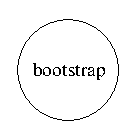
\includegraphics{figures/k0.eps}}
\end{figure}

\newpage

\subsubsection{k1}

\paragraph{}

Le projet s'\'etale sur \textbf{deux} semaines.

\paragraph{}

L'\'etudiant disposera de \textbf{quatre} heures de cours et de \textbf{six}
heures de travaux pratiques.

\paragraph{}

Le but du projet est le d\'eveloppement d'un bootloader.
Celui ci devra mettre en place un nouveau mode d'adressage et installer
une configuration m\'emoire satisfaisante pour la future ex\'ecution du kernel.

\paragraph{}

\`A travers ce projet, l'\'etudiant aura l'occasion d'acqu\'erir de nouvelles
notions processeurs et de les appliquer. Ce projet introduit la notion
de m\'emoire virtuelle, une notion fondamentale pour la suite du projet
\textbf{kaneton}.

\vspace{5cm}

\begin{figure}[h]
\centerline{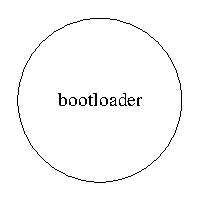
\includegraphics{figures/k1.eps}}
\end{figure}

\newpage

\subsubsection{k2}

\paragraph{}

Le projet s'\'etale sur \textbf{quatres} semaines.

\paragraph{}

L'\'etudiant disposera de \textbf{quatre} heures de cours et de \textbf{douze}
heures de travaux pratiques.

\paragraph{}

Le but du projet est le lancement du kernel et la mise en place d'un certain
nombre de gestionnaires: espaces d'adressage, m\'emoire physique,
interruptions etc.. et certains pilotes basiques: timer, PIC, console,
clavier etc..

\paragraph{}

Ce projet est une des tranches les plus importantes du projet et ne devra
pas \^etre pris \`a la l\'eg\`ere.

\paragraph{}

L'\'etudiant via ce projet aura l'occasion de se familiariser avec le
fonctionnement des communications avec les p\'eriph\'eriques, la notion de
temps, et le d\'eveloppement de pilotes basiques mais surtout les
probl\'ematiques li\'ees \`a la portabilit\'e.

\vspace{5cm}

\begin{figure}[h]
\centerline{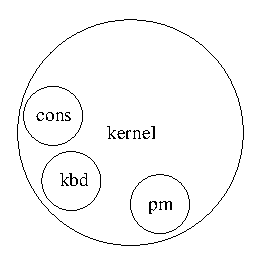
\includegraphics{figures/k2.eps}}
\end{figure}

\newpage

\subsection{KAN2: Gestion de l'ex\'ecution}

\paragraph{}

\subsubsection{k3}

\paragraph{}

Le projet s'\'etale sur \textbf{deux} semaines.

\paragraph{}

L'\'etudiant disposera de \textbf{quatre} heures de cours et de \textbf{six}
heures de travaux pratiques.

\paragraph{}

Le but du projet est la mise en place du gestionnaire de m\'emoire virtuelle.

\paragraph{}

L'\'etudiant confortera durant cette p\'eriode ses acquis vis-\`a-vis du
fonctionnement interne du processeur.

\vspace{5cm}

\begin{figure}[h]
\centerline{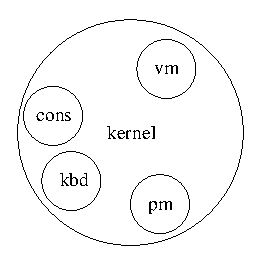
\includegraphics{figures/k3.eps}}
\end{figure}

\newpage

\subsubsection{k4}

\paragraph{}

Le projet s'\'etale sur \textbf{cinq} semaines.

\paragraph{}

L'\'etudiant disposera de \textbf{quatre} heures de cours et de \textbf{quinze}
heures de travaux pratiques.

\paragraph{}

Le but du projet est la mise en place du gestionnaire de processus avec
gestion des threads, de l'ordonnanceur, mais \'egalement d'un gestionnaire
d'ensembles et d'un gestionnaire de modules.

\paragraph{}

Ce projet est tr\`es certainement le plus important de tous.

\paragraph{}

L'\'etudiant aura l'occasion d'acqu\'erir de nouvelles notions processeur
mais \'egalement de d\'evelopper des interfaces complexes mais coh\'erentes
pour permettre la gestion des processus.

\vspace{5cm}

\begin{figure}[h]
\centerline{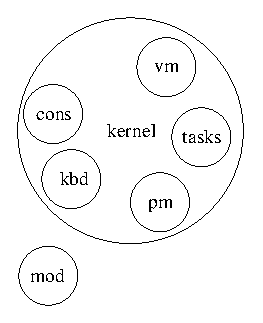
\includegraphics{figures/k4.eps}}
\end{figure}

\newpage

\subsection{KAN3: Communications et Ressources}

\paragraph{}

\subsubsection{k5}

\paragraph{}

Le projet s'\'etale sur \textbf{deux} semaines.

\paragraph{}

L'\'etudiant disposera de \textbf{trois} heures de cours et de \textbf{six}
heures de travaux pratiques.

\paragraph{}

Le but du projet est le d\'eveloppement d'un syst\`eme de communication
inter-processus.

\paragraph{}

L'\'etudiant aura l'occasion de d\'ecouvrir les diff\'erentes techniques
connues pour mettre en place la communication et les probl\`emes
d'impl\'ementation connus.

\vspace{5cm}

\begin{figure}[h]
\centerline{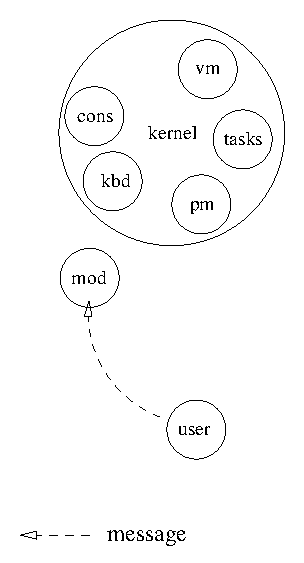
\includegraphics{figures/k5.eps}}
\end{figure}

\newpage

\subsubsection{k6}

\paragraph{}

Le projet s'\'etale sur \textbf{trois} semaines.

\paragraph{}

L'\'etudiant disposera de \textbf{trois} heures de cours et de \textbf{neuf}
heures de travaux pratiques.

\paragraph{}

Le but du projet est le d\'eveloppement d'un pilote IDE et d'un
gestionnaire des partitions.

\paragraph{}

L'\'etudiant se confronter cette fois-ci au d\'eveloppement d'un pilote
bien plus complexe et devra faire face \`a cette difficult\'e en se
documentant correctement sur les m\'ecanismes bas niveau utilis\'es.

\vspace{5cm}

\begin{figure}[h]
\centerline{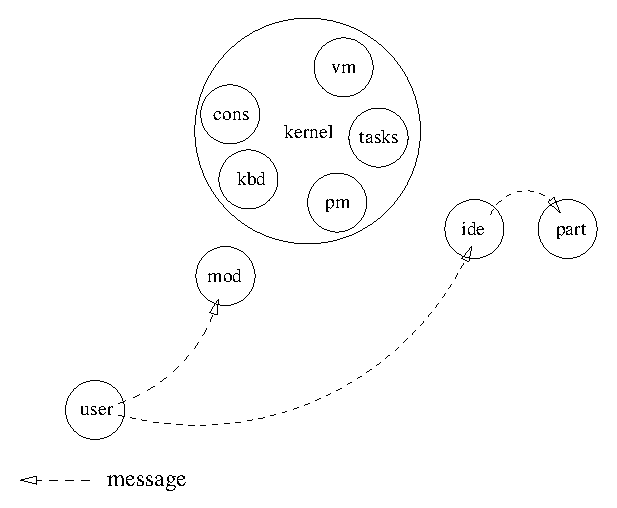
\includegraphics{figures/k6.eps}}
\end{figure}

\newpage

\subsubsection{k7}

\paragraph{}

Le projet s'\'etale sur \textbf{deux} semaines.

\paragraph{}

L'\'etudiant disposera de \textbf{deux} heures de cours et de \textbf{six}
heures de travaux pratiques.

\paragraph{}

Le but du projet est de concevoir enti\`erement un syst\`eme et de
l'impl\'ementer. L'objet du projet est le d\'eveloppement d'un gestionnaire
de p\'eriph\'eriques.

\paragraph{}

L'\'etudiant devra faire face \`a toute une phase de r\'eflexion li\'ee
\`a la conception suivie de l'\'etablissement d'un dossier de sp\'ecification.
L'\'etudiant jouera donc un double r\^ole, celui de l'architecte et celui
du d\'eveloppeur.

\vspace{5cm}

\begin{figure}[h]
\centerline{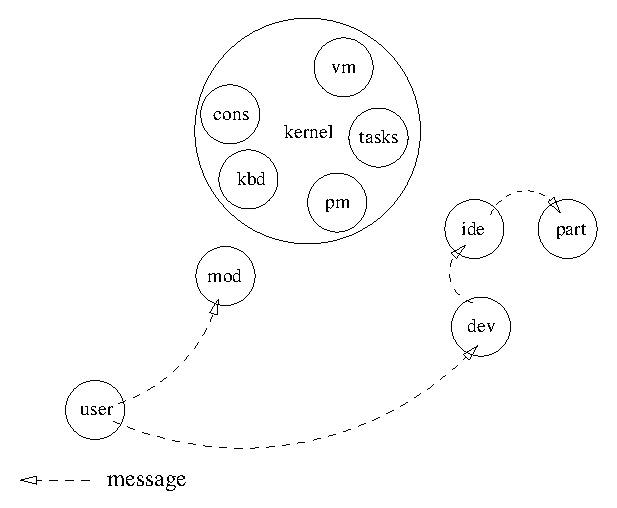
\includegraphics{figures/k7.eps}}
\end{figure}

\newpage

\subsection{KAN4: Syst\`emes de fichiers}

\paragraph{}

\subsubsection{k8}

\paragraph{}

Le projet s'\'etale sur \textbf{quatre} semaines.

\paragraph{}

L'\'etudiant disposera de \textbf{quatre} heures de cours et de \textbf{douze}
heures de travaux pratiques.

\paragraph{}

Le but du projet est de concevoir et impl\'ementer un syst\`eme de fichiers
basique.

\paragraph{}

L'\'etudiant aura l'occasion d'\'etudier le fonctionnement des syst\`emes
de fichiers anciens tout comme modernes et d'en d\'evelopper un.

\vspace{5cm}

\begin{figure}[h]
\centerline{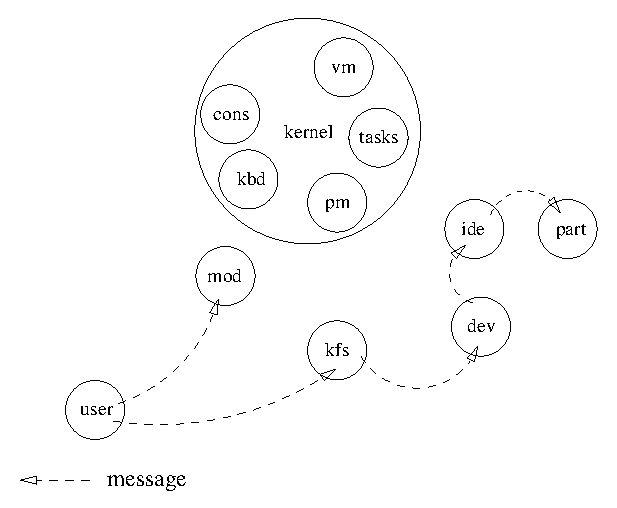
\includegraphics{figures/k8.eps}}
\end{figure}

\newpage

\subsubsection{k9}

\paragraph{}

Le projet s'\'etale sur \textbf{deux} semaines.

\paragraph{}

L'\'etudiant disposera de \textbf{trois} heures de cours et de \textbf{six}
heures de travaux pratiques.

\paragraph{}

Le but du projet est de d\'evelopper un syst\`eme de fichiers virtuel VFS
et un syst\`eme de fichiers situ\'e en m\'emoire principale ModFS.

\paragraph{}

L'\'etudiant aura donc la possibilit\'e d'\'etudier le fonctionnement
d'une interface g\'en\'erique, dans notre cas VFS.

\vspace{5cm}

\begin{figure}[h]
\centerline{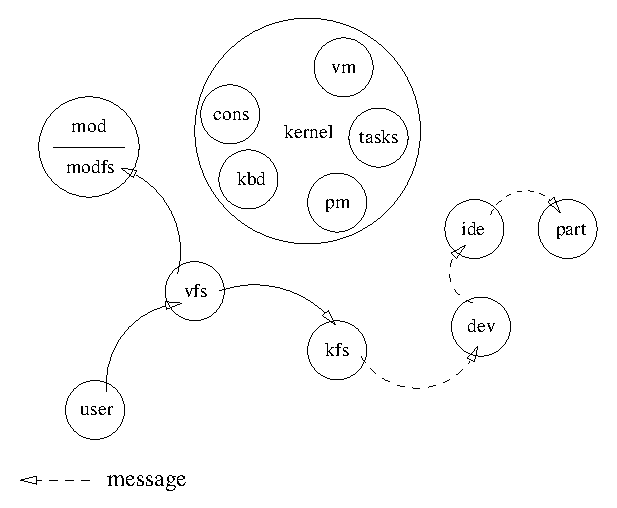
\includegraphics{figures/k9.eps}}
\end{figure}

\newpage

\subsubsection{k10}

\paragraph{}

Le projet s'\'etale sur \textbf{deux} semaines.

\paragraph{}

L'\'etudiant disposera de \textbf{deux} heures de cours et de \textbf{six}
heures de travaux pratiques.

\paragraph{}

Le but du projet est de d\'evelopper une partie du syst\`eme librement.
L'\'etudiant devra donc \'etablir un cahier des charges, des sp\'ecifications
et impl\'ementer sa conception.

\vspace{5cm}

\begin{figure}[h]
\centerline{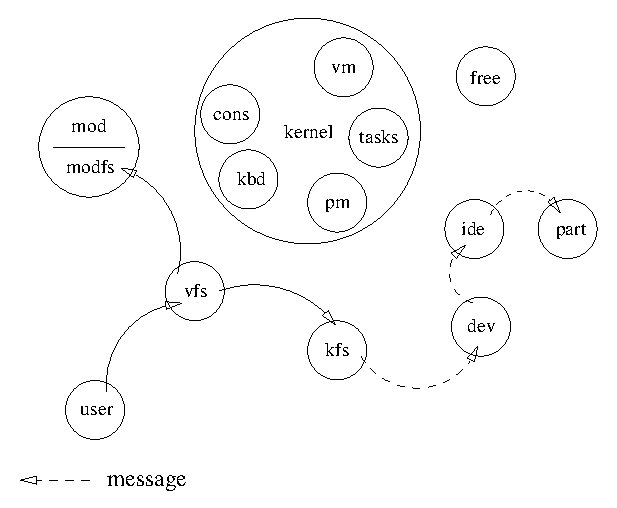
\includegraphics{figures/k10.eps}}
\end{figure}

\newpage

\section{D\'eroulement d'un projet}

Chaque projet se d\'eroule de la facon suivante:

\begin{enumerate}

\item \textbf{Pr\'esentation du projet}: explication des objectifs \`a
      atteindre, des notions \`a acqu\'erir, de la mod\'elisation propos\'ee
      etc..

\item \textbf{Tp}: durant le projet, des TPs seront organis\'es,
      g\'en\'eralement une sc\'eance toute les semaines, afin que vous
      puissiez poser vos questions.

\item \textbf{Soutenance}: \`a l'issue de chaque p\'eriode de projet, une
      soutenance aura lieu afin d'\'evaluer le travail du groupe. Attention,
      la notation sera bas\'ee sur les r\'eponses de chaque membre du groupe.
      En d'autres termes, si plusieurs personnes dans le groupe ne savent
      pas r\'epondre la note s'en verra recalcul\'ee.

\item \textbf{Partiel}: un partiel aura lieu pour valider vos connaissances
      sur la totalit\'e des notions vues jusque l\`a.

\end{enumerate}

\paragraph{}

Il est important de savoir qu'aucun support de cours ne sera fourni. La
pr\'esentation du projet inclus un cours sur les notions \`a comprendre
et \`a connaitre. Les \'etudiants sont donc fortement invit\'es \`a
assister aux cours et \`a prendre des notes pour ne pas perdre de temps
durant le d\'eveloppement du projet.

\paragraph{}

Le sujet sera le seul document fourni et contiendra en plus de la description
du projet, la liste des documentations \`a lire pour r\'eussir le projet.
Bien entendu, l'\'etudiant qui aura assimil\'e les notions abord\'ees en
cours n'aura quasiment aucun document \`a lire.

\paragraph{}

Certains projets sont destin\'es \`a initier les \'etudiants \`a la
mod\'elisation noyau. Dans ces projets particuliers, nous
vous invitons \`a suivre notre mod\'elisation. N\'eanmoins vous
pourrez tout \`a fait prendre la d\'ecision d'impl\'ementer votre
propre mod\'elisation. Dans ce cas, vous devrez nous fournir une documentation
claire et pr\'ecise expliquant vos choix. Si votre mod\'elisation est
intelligente et apporte des inovations par rapport \`a celle fournie,
votre note se verra amelior\'ee et votre mod\'elisation pourrait devenir
celle que nous proposerons pour les ann\'ees suivantes.

\paragraph{}

Attention, il vous faudra tout de m\^eme fournir une couche de compatibilit\'e
avec notre mod\'elisation pour permettre \`a notre moulinette de passer.

\end{document}
